\begin{frame}
	\begin{minipage}[t][0.6\textheight][t]{\textwidth}
		\begin{columns}
			\column{0.5\textwidth}
			\begin{overlayarea}{\textwidth}{\textheight}
				\only<1->{\myheading{Better Activation Functions}}
				\justify
				\only<1>{The \textbf{logistic function} was the most popular choice in the 80's }
				\only<2>{The \textbf{tanh function} which is zero centered leads to better convergence
					\cite{LeCun:91}}
				\only<3->{ More recently it has been shown that \textbf{Rectified Linear Units (ReLUs)} and their variants lead to better performance \cite{Nair2010}, \cite{Krizhevsky:2012},\cite{Maas2013}}
			\end{overlayarea}
			\column{0.5\textwidth}
			\begin{overlayarea}{\textwidth}{\textheight}
				\begin{figure}
					\centering
					\only<1>{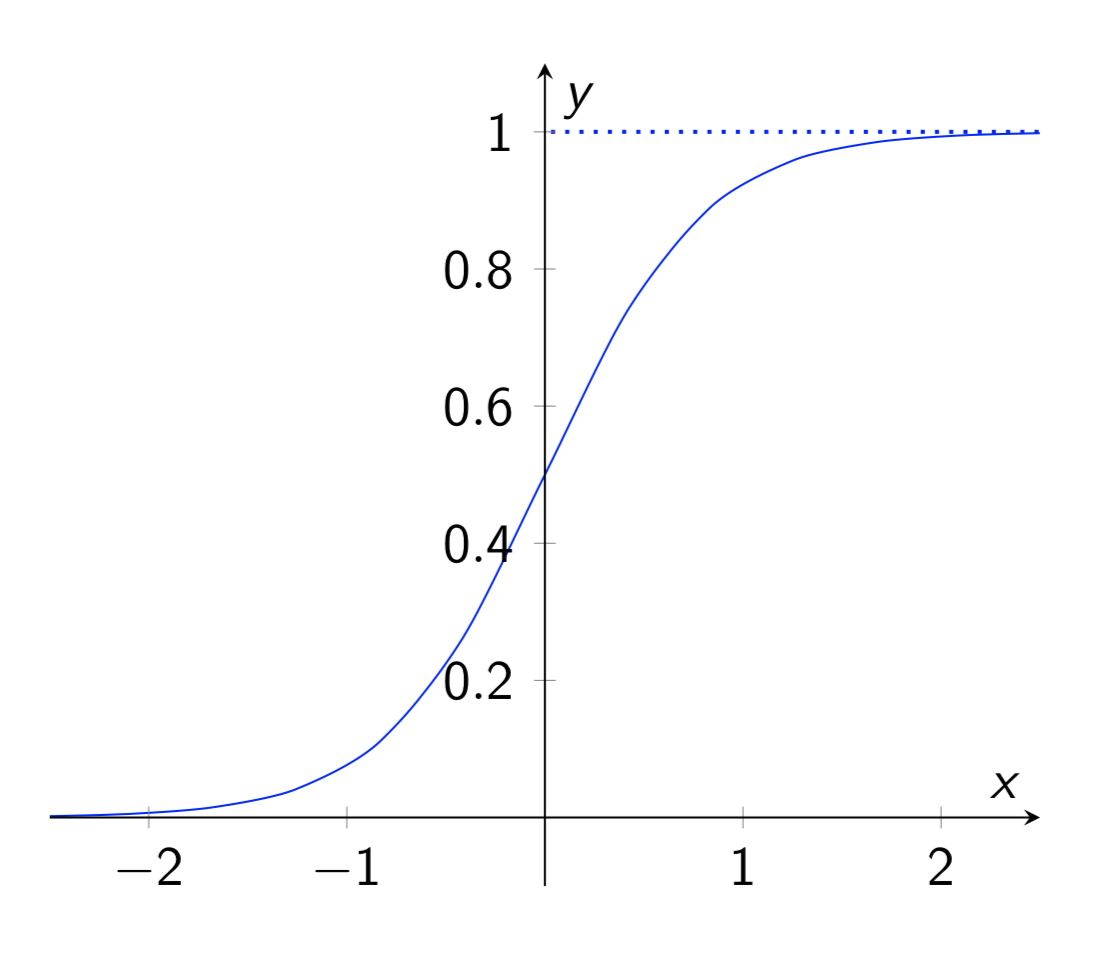
\includegraphics[scale=0.2]{images/module5/logistic}}
					\only<2>{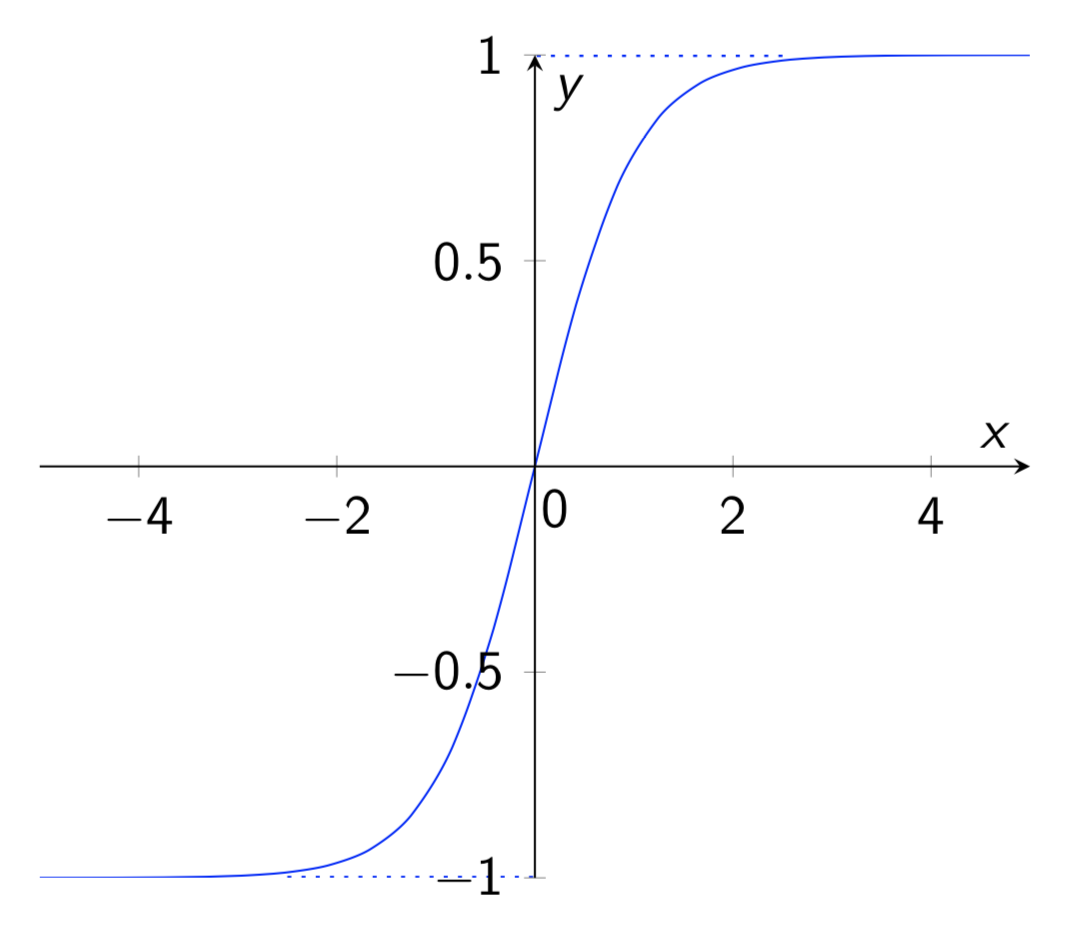
\includegraphics[scale=0.2]{images/module5/tanh}}
					%\only<3>{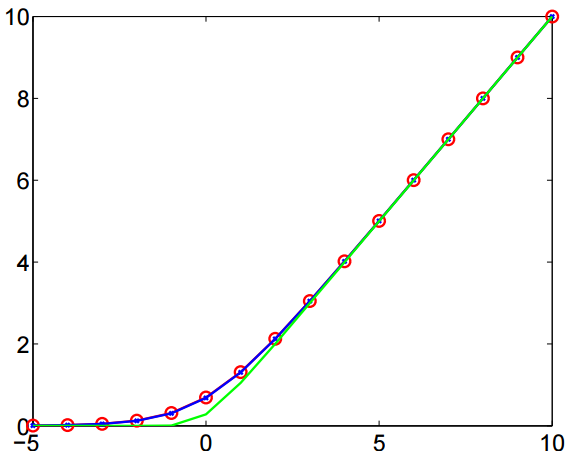
\includegraphics[scale=0.2]{images/relu_rbm}}
					%\only<4>{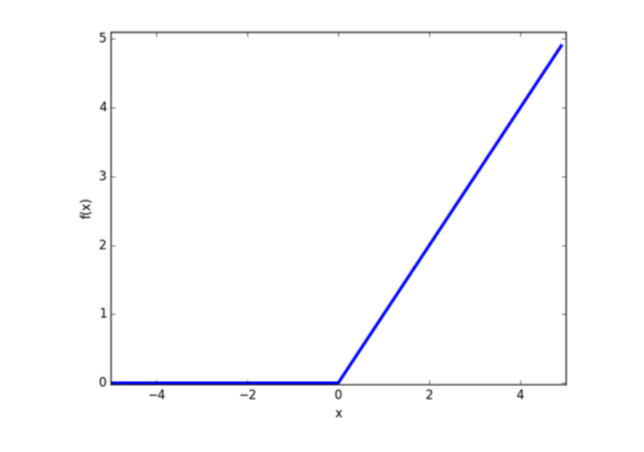
\includegraphics[scale=0.5]{images/relu_cnn}}
					\only<3->{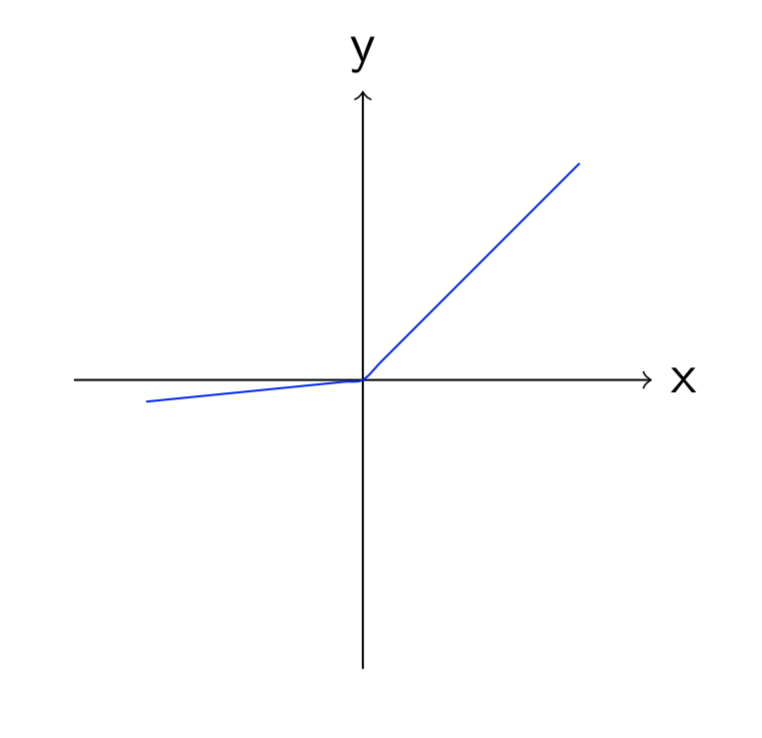
\includegraphics[scale=0.4]{images/module5/leaky_relu}}
					%\only<6>{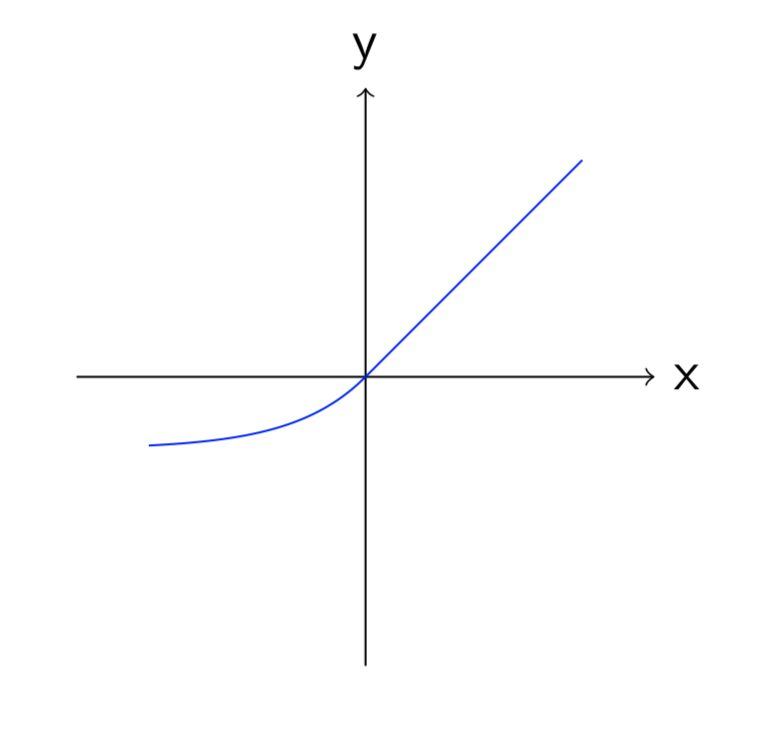
\includegraphics[scale=0.4]{images/exponential_relu}}
					%\only<7>{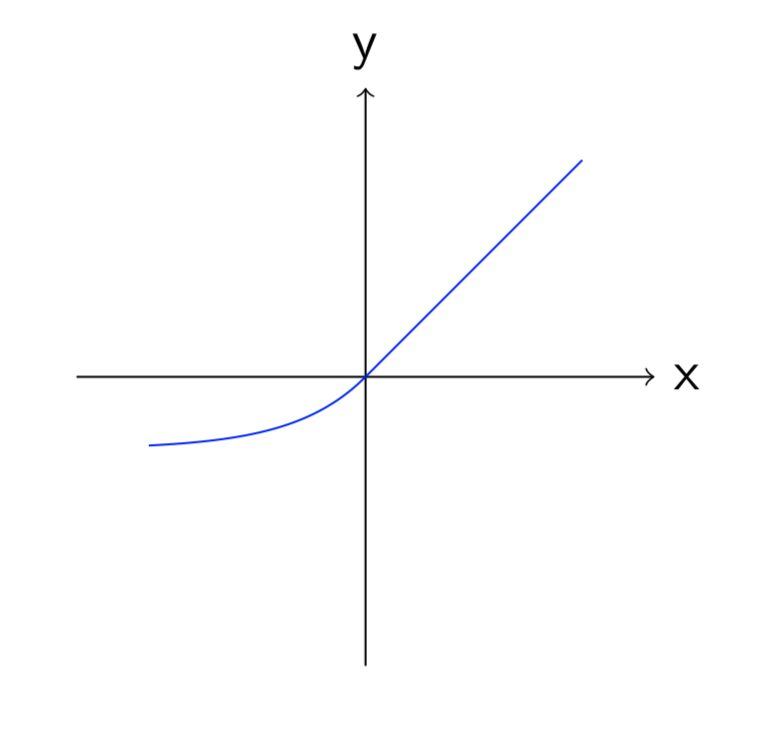
\includegraphics[scale=0.4]{images/exponential_relu}}
				\end{figure}
			\end{overlayarea}
		\end{columns}
	\end{minipage}
	\begin{minipage}[t][0.4\textheight][t]{\textwidth}
		\begin{overlayarea}{\textwidth}{\textheight}
			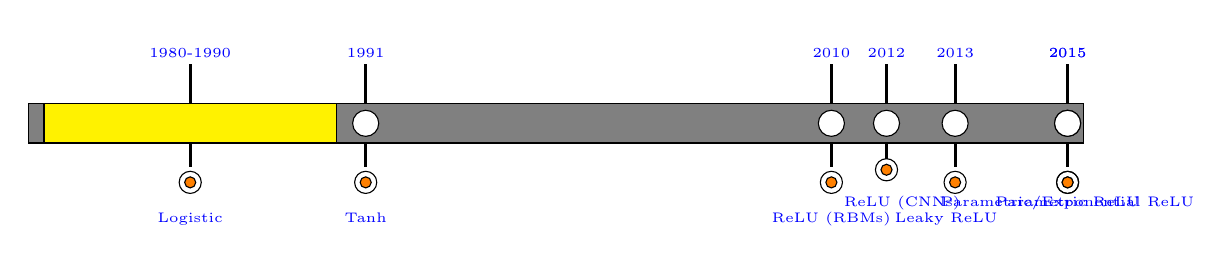
\begin{tikzpicture}[datemarker/.style={circle, draw=black,fill=white},textlabel/.style={anchor=center,text height=1.7ex,text depth=.25ex}]
				\tikzset{every node/.style={font=\tiny, color=blue}}\draw[fill=gray](-0.2,0) rectangle (13.2,0.5) node[white, below]{};
				\onslide<1->{\draw[fill=yellow](0.0,0) rectangle (3.71428571429, 0.5){};}
				\onslide<1->{\draw [line width=1pt] (1.85714285714, 0.5) to (1.85714285714, 1.0);}
				\onslide<1->{\draw (1.85714285714, 1.2) node [textlabel]{1980-1990};}
				\onslide<1->{\draw [fill=orange](1.85714285714, -0.5) circle (2pt){};}
				\onslide<1->{\draw(1.85714285714, -0.5) circle (4pt){};}
				\onslide<1->{\draw [line width=1pt] (1.85714285714, 0) to (1.85714285714, -0.3);}
				\onslide<1->{\draw (1.85714285714,-0.9) node [textlabel] {Logistic};}
				\onslide<2->{\node at (4.08571428571, 0.25) [datemarker] {};}
				\onslide<2->{\draw [line width=1pt] (4.08571428571, 0.5) to (4.08571428571, 1.0);}
				\onslide<2->{\draw (4.08571428571, 1.2) node [textlabel]{1991};}
				\onslide<2->{\draw [fill=orange](4.08571428571, -0.5) circle (2pt){};}
				\onslide<2->{\draw(4.08571428571, -0.5) circle (4pt){};}
				\onslide<2->{\draw [line width=1pt] (4.08571428571, 0) to (4.08571428571, -0.3);}
				\onslide<2->{\draw (4.08571428571,-0.9) node [textlabel] {Tanh};}

				\onslide<3->{\node at (10, 0.25) [datemarker] {};}
				\onslide<3->{\draw [line width=1pt] (10, 0.5) to (10, 1.0);}
				\onslide<3->{\draw (10, 1.2) node [textlabel]{2010};}
				\onslide<3->{\draw [fill=orange](10, -0.5) circle (2pt){};}
				\onslide<3->{\draw(10, -0.5) circle (4pt){};}
				\onslide<3->{\draw [line width=1pt] (10, 0) to (10, -0.3);}
				\onslide<3->{\draw (10,-0.9) node [textlabel] {ReLU (RBMs)};}
				\onslide<4->{\node at (10.7, 0.25) [datemarker] {};}
				\onslide<4->{\draw [line width=1pt] (10.7, 0.5) to (10.7, 1.0);}
				\onslide<4->{\draw (10.7, 1.2) node [textlabel]{2012};}
				\onslide<4->{\draw [fill=orange](10.7, -0.34) circle (2pt){};}
				\onslide<4->{\draw(10.7, -0.34) circle (4pt){};}
				\onslide<4->{\draw [line width=1pt] (10.7, 0) to (10.7, -0.2);}
				\onslide<4->{\draw (10.9,-0.7) node [textlabel] {ReLU (CNNs)};}
				\onslide<5->{\node at (11.571428571, 0.25) [datemarker] {};}
				\onslide<5->{\draw [line width=1pt] (11.571428571, 0.5) to (11.571428571, 1.0);}
				\onslide<5->{\draw (11.571428571, 1.2) node [textlabel]{2013};}
				\onslide<5->{\draw [fill=orange](11.571428571, -0.5) circle (2pt){};}
				\onslide<5->{\draw(11.571428571, -0.5) circle (4pt){};}
				\onslide<5->{\draw [line width=1pt] (11.571428571, 0) to (11.571428571, -0.3);}
				\onslide<5->{\draw (11.4571428571,-0.9) node [textlabel] {Leaky ReLU};}
				\onslide<6->{\node at (13.0, 0.25) [datemarker] {};}
				\onslide<6->{\draw [line width=1pt] (13.0, 0.5) to (13.0, 1.0);}
				\onslide<6->{\draw (13.0, 1.2) node [textlabel]{2015};}
				\onslide<6->{\draw [fill=orange](13.0, -0.5) circle (2pt){};}
				\onslide<6->{\draw(13.0, -0.5) circle (4pt){};}
				\onslide<6->{\draw [line width=1pt] (13.0, 0) to (13.0, -0.3);}
				\onslide<6>{\draw (13.0,-0.7) node [textlabel] {Parametric ReLU};}
				\onslide<7->{\node at (13.0, 0.25) [datemarker] {};}
				\onslide<7->{\draw [line width=1pt] (13.0, 0.5) to (13.0, 1.0);}
				\onslide<7->{\draw (13.0, 1.2) node [textlabel]{2015};}
				\onslide<7->{\draw [fill=orange](13.0, -0.5) circle (2pt){};}
				\onslide<7->{\draw(13.0, -0.5) circle (4pt){};}
				\onslide<7->{\draw [line width=1pt] (13.0, 0) to (13.0, -0.3);}
				\onslide<7->{\draw (13.0,-0.7) node [textlabel] {Parametric/Exponential ReLU};}
			\end{tikzpicture}
		\end{overlayarea}
	\end{minipage}
\end{frame}
